\documentclass[tikz]{standalone}
\usepackage{tikz}
\usepackage{amsmath}

\renewcommand\familydefault{\sfdefault}

\begin{document}
\large

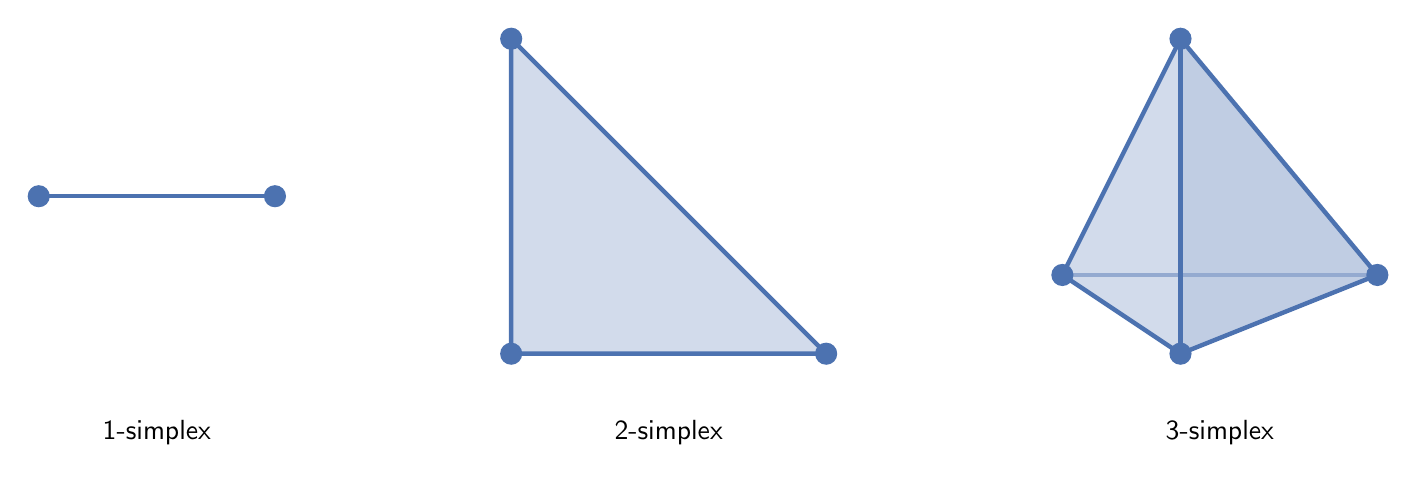
\begin{tikzpicture}[scale=2]
\definecolor{VertexBlue}{HTML}{4C72B0};
\definecolor{LineBlue}{HTML}{4C72B0};
\definecolor{FaceBlue}{HTML}{D2DBEB};
\definecolor{FaceDarkBlue}{HTML}{C0CDE3};

% 1-simplex
\begin{scope}[shift={(0, 0)}]
\draw[LineBlue, ultra thick] (0, 1) -- (1.5, 1);
\fill[VertexBlue] (0, 1) circle (2pt);
\fill[VertexBlue] (1.5, 1) circle (2pt);
\node at (0.75, -0.5) {1-simplex};
\end{scope}

% 2-simplex
\begin{scope}[shift={(3, 0)}]
\coordinate (A) at (0, 0);
\coordinate (B) at (2, 0);
\coordinate (C) at (0, 2);

\fill[FaceBlue] (A) -- (B) -- (C) -- cycle;
\draw[LineBlue, ultra thick] (A) -- (B) -- (C) -- cycle;
\foreach \p in {A,B,C}
    \fill[VertexBlue] (\p) circle (2pt);

\node at (1, -0.5) {2-simplex};
\end{scope}

% 3-simplex
\begin{scope}[shift={(6.5, 0)}]
\coordinate (O) at (0, 0.5, 0);
\coordinate (X) at (2, 0.5, 0);
\coordinate (Y) at (0.75, 2, 0);
\coordinate (Z) at (0.75, 0.0, 0.0);

% faces
\fill[FaceBlue] (O) -- (X) -- (Y) -- cycle;
\fill[FaceBlue] (O) -- (X) -- (Z) -- cycle;
\fill[FaceDarkBlue] (X) -- (Y) -- (Z) -- cycle;
\fill[FaceBlue] (Y) -- (O) -- (Z) -- cycle;

% edges
\draw[LineBlue, ultra thick] (X) -- (Y) -- (O);
\draw[LineBlue!60, ultra thick] (O) -- (X);
\draw[LineBlue, ultra thick] (O) -- (Z);
\draw[LineBlue, ultra thick] (X) -- (Z);
\draw[LineBlue, ultra thick] (Y) -- (Z);

% vertices
\foreach \p in {O,X,Y,Z}
    \fill[VertexBlue] (\p) circle (2pt);

\node at (1, -0.5, 0) {3-simplex};
\end{scope}
\end{tikzpicture}

\end{document}
